\subsection{Inputs and outputs of the NN}

After reading the original paper~\cite{turaga_maximin_2009} we realized that
there was some missing information on implementation details.
One of the most important points, the input and the output of the neural
network, was not clear. After some research we were lucky to find Srinivas
Turaga's Phd thesis~\cite{turaga_learning_2010}. In it MALIS was presented in
more details, especially the neural network used in the experiments.\\

The network predicts the affinity following each axis. As we can see in
figure~\ref{fig:nn_output}, in the case where the network is fed a 3D image, it
outputs three affinity images following the axis X, Y and Z. Then we have to
merge these three images in a way to obtain the complete affinity graph.

\begin{figure}[!htbp]
	\centering
	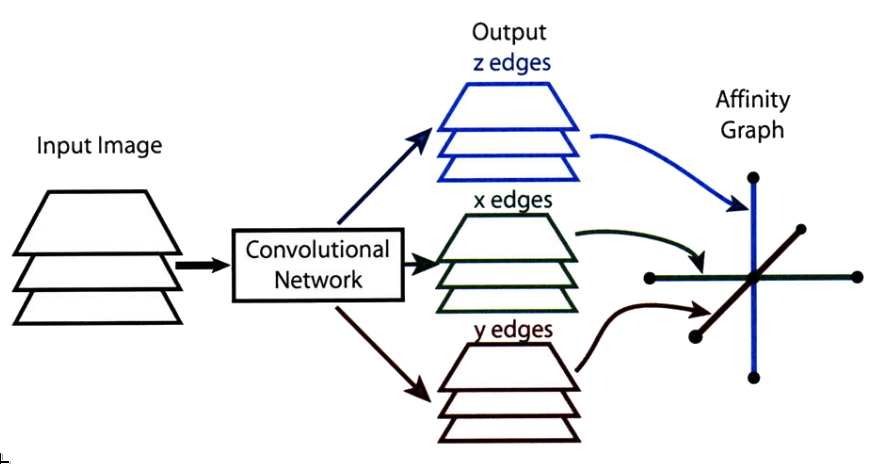
\includegraphics[width=0.8\linewidth]{./images/nn_output.png}
	\caption{Creating the affinity graph using a convolutional network. The
	input to the network is the 3d EM image and the desired output is a set of
3d images: one each for the x, y and z directions representing the affinity
graph, from~\cite{turaga_learning_2010}}%
	\label{fig:nn_output}
\end{figure}

Another problem was to understand the input shape. In the paper, they use a
patch size of $21\times21\times21$. But it is also said that it led to an affinity
classifier that uses a patch with a shape of $17\times17\times17$ to classify an affinity
edge. At first it was kind of blur but we figured out that 17 correspond
to the volume taking in account after four convolution layers with a kernel
size of $5\times5$, reminiscent to the proposed architecture. The patch size is also arbitrary as we are using a FCN that, by definition, don’t care about the input shape.\\

\subsection{Computing the maximin edge}

As said earlier, we have to find the maximin edge in order to compute the loss.
As we have to do this operation for each training iteration, it is very important to
guarantee a very low computational cost. Our first approach was to use the
Breadth First Search algorithm on the Maximum Spanning Tree efficiently created
with Higra. Sadly, this method was not good because our implementation was
suffering from the slowness of Python and its $\mathcal{O}(n)$ complexity for each pair of
pixel, which scales badly with the number of pairs chosen. \\

\begin{figure}[!htbp]
	\centering
	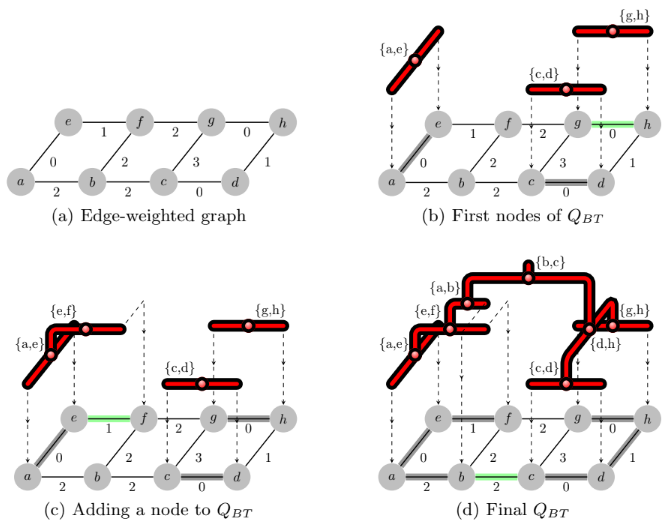
\includegraphics[width=0.7\linewidth]{./images/bpt.png}
	\caption{A simple process for obtaining a binary tree providing a strict
	total order relation on the edges of the MST, from~\cite{najman_playing_2013}}%
	\label{fig:bpt_method}
\end{figure}


In our last version we are computing a Binary Partition Tree, a binary tree by
altitude ordering. This tree is build using Kruskal algorithm. The way to build
this tree is straightforward, as illustrated in figure~\ref{fig:bpt_method}. 
Edges are added to the tree in order of altitude as our MST is built, as
described in \cite{najman_playing_2013}.
This data structure is pretty pertinent as the
maximin edge between two pixels $i$ and $j$ is the lowest common ancestor of these
two pixels in the BPT. Higra also allows us to compute the loss with a larger
number of pairs without an explosion of computing time because picking the
lowest common ancestor is achieved in constant time, with a preprocessing in
$\mathcal{O}(n\log(n))$.

\subsection{Interaction between Higra and PyTorch}

We had some trouble with the interaction between Higra and Pytorch. In order to
compute the loss, we have to compute a BPT on a graph build from the NN output
to find the maximin edge used in the loss computation. As you can see in
figure~\ref{fig:bpt_method}, the gradient history is lost by turning the
affinities images in graph using Higra.\\
We were unable to keep tracking the gradient history by working on
graphs, even after a thorough examination of each step of the process. 
Therefore it was impossible to train our model. But without Higra the
training would be much longer. And even the previous technique using the
Breadth First Search would not work as we are using Higra to compute the MST.
We found the solution in a code proposed by Giovanni Chierchia and Benjamin
Perret in~\cite{chierchia_ultrametric_2019} for computing the subdominant
ultrametric, which is analogous to our problem. Higra has a function that
allows us to make the correspondance between an edge in the graph and the output
affinity image. Consequently, we are able to localise the maximin edge in the
output image. Due to the fact that picking an edge does not cause gradient
history loss we are done.

\begin{figure}[!htbp]
	\centering
	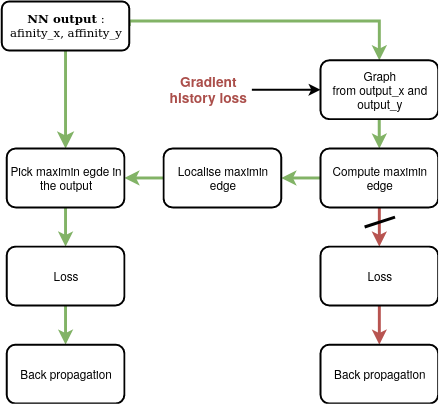
\includegraphics[width=0.6\linewidth]{./images/gradient_history.png}
	\caption{Process to compute the loss from our neural network. The red path
	was our first idea but proved unsuccesful. The green path represents the
process we are using currently.}
	\label{fig:bpt_method}
\end{figure}


